

\title{Machine learning inference of search engine heuristics}
\subtitle{Part II Computer Science Project Proposal}
\author{K. Palyutina, St. Catharine's College \\
        Originator: Dr. Jon Crowcroft}
\maketitle


\vfil


\noindent
{\bf Project Supervisor:} Prof. J. Crowcroft
\vspace{0.2in}

\noindent
{\bf Director of Studies:} Dr. S. Taraskin
\vspace{0.2in}
\noindent
 
\noindent
{\bf Project Overseers:} Dr.~M.~Kuhn  \& Dr~A.~Madhavapeddy


% Main document

\section*{\bf Introduction, The Problem To Be Addressed}
PageRank (an algorithm which is used by Google to evaluate the `importance' of a web page) is one of the most crucial factors which determine page performance in search returns. However, there are many more of such factors that are believed to become increasingly influential. Because Google's algorithm is frequently revised, changing page ranks cause web site owners to speculate about how their web pages `deserved' an upgrade or a downgrade. Despite a large interest in this area, little research has been done to determine to what degree such factors affect the performance of a page. Certain tools\footnote{For example, Woorank or SEO are the most popular Chrome extensions to assess certain page qualities.} exist which attempt to advise web masters how to `improve' their pages. However, heuristics used by such tools are not known and are possibly incomplete and no attempt has come close to accurately predicting Google rankings.

A problem of approximating algorithms which may be used by modern search engines is characterised by vast search space, which makes exhaustive search impossible and introduces the need for generalisation. Such a problem can be reduced to a classification problem, which is traditionally solved with the help of machine learning techniques. Even though machine learning finds natural application in this area, it is easy to see how it would be very hard to create a learner and apply it to, for example, Google's search engine. Naturally, one would need to have exhaustive resources to conduct such a study. Besides, machine learning has major drawbacks that would hinder such an ambitious experiment.

Firstly, there are little theoretical guarantees in this approach. Bounds, if any, referring to how much data needs to be processed to produce a `correct' classifier are very imprecise and a classifier that performs well in practice may not be `true'\footnote{A classifier is `true' if it classifies data correctly for all inputs.}. This means that if a machine learner was to be trained by the `real world' data (Google search returns), little could be said about the performance of the obtained algorithm or, indeed, the `truthfulness' of it. Not only would it give little insight into how successful the learning is, but also no guidance for improvement. 

Another similar issue is referred to as `overfitting': this describes a situation in which a classifier performs outstandingly on a particular set of data (often similar to training data), but given different data will perform as badly as random selection. This occurs when false connections between features and outputs have been made by the learner. Unfortunately, there is no single technique that will always avoid over/under-fitting\cite{domingos}.

Clearly, such limitations are hard to combat. Besides, machine learning techniques vary greatly, so clear and detailed feedback is essential to draw conclusions about the performance of a learner. Knowing how a particular technique copes with certain heuristics would be valuable, as it would allow to approach the original problem (approximating search engine heuristics reliably) in an informed way.  

In this light, this project aspires to explore how machine learning techniques can be used to infer algorithms from search engines. To battle the constraints described above I will write my own simple search engine which will be used to observe the effectiveness of different machine learning techniques (see Figure \ref{diag1}). The existence of such a search engine is vital to the project, as it offers ultimate control over the learning process. The heuristics used in the search engine will be transparent, which, for example, eliminates the dependency on continuously changing heuristics used by Google. Another advantage of this approach is the fact that only a minimal fraction of the web needs to be used. Such a `mini-internet' will reside offline, which will speed up the indexing and also allow local modification of web pages. 

\begin{figure}
\centering
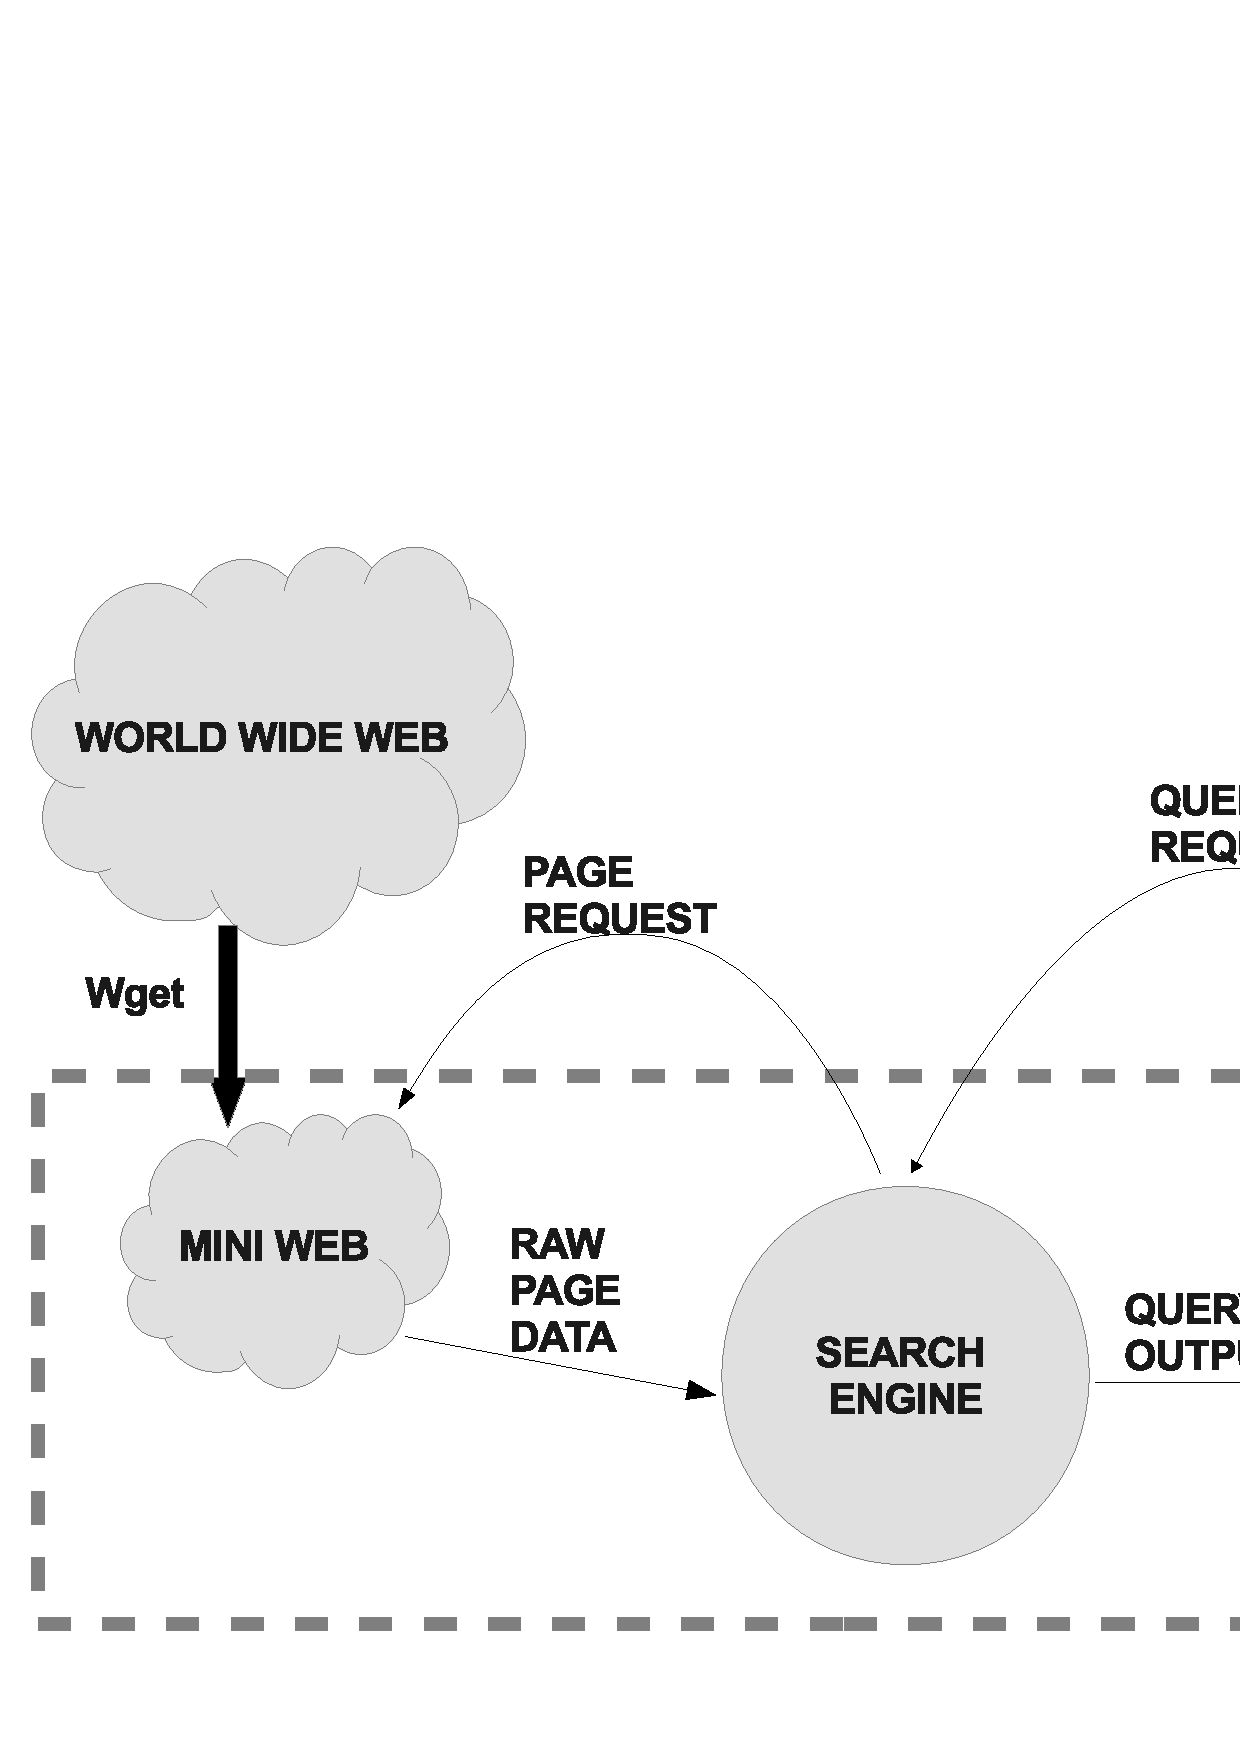
\includegraphics[scale=0.5]{diagram1}
\caption{The training of the learner. The system enclosed within the dotted box will be implemented in this project. The mini web is created by cloning web pages from the internet. The learner queries the search engine and gets back the results of the query as an input. }
\label{diag1}
\end{figure}

Most importantly, this approach gives me straightforward ways to reason about the performance of learning techniques. The search engine can be evolved to incorporate various heuristics together with PageRank. Such heuristics need not match Google's actual heuristics, however must aim to improve browsing experience \footnote{`Precision and Recall' method can be used as a guide to evaluation of search engine complexity.}. A lot of speculation has been done by web masters as to which qualities of a web page affect its ranking, these include compliance with web standards, number of words per page, frequency of occurrence of the search term on the page and alike. Because the goal of the project does not include `reverse engineering' any particular existing algorithm, there is no harm in using such guesses as guidance. 

Evolving the search engine and, hence, the learner iteratively will result in comprehensive conclusions about the effectiveness of the machine learning technique in question. Such conclusions can be used in the future as a guidance to learner design. 

\section*{\bf Starting Point}

\begin{itemize}
\item A project\cite{reid} was undertaken by the proposer, which developed a primitive algorithm to predict, given six characteristics of a web page, its Google ranking.  This project is mainly an inspiration, however, the speculations about the Google page ranking factors can be useful for the search engine design. 
\item Python packages exist for manipulating web pages.
\item Wget is a Linux open source utility that can be used to clone web pages.
\item The paper describing PageRank is published and will be used to implement the algorithm.
\end{itemize}


\section*{\bf Resources Required}
\begin{itemize}
\item For this project I shall mainly use my own dual-core computer that runs Ubuntu Linux. I accept full responsibility for this machine and I have made contingency plans to protect myself against hardware and/or software failure.
\item Backup will be to a Bitbucket repository and/or an external hard drive.
\item I will work on MCS computers should my main machine suddenly fail. 
\end{itemize}
\section*{\bf Work to be done}

The project breaks down into the following sub-projects:

\begin{enumerate}
\item Decide on a category of search terms to explore in order to create a small network consisting of relevant web pages.

\item Implement PageRank within this network. 

\item Write a simple search engine incorporating PageRank and few other features. 

\item Decide on the representation of the input for the learner and set up the framework to format it. 

\item In advance set aside training and test data: this is necessary to then justify the evaluation of the classifier.

\item Write a simple prototype for the learner\footnote {A Naive Bayesian would be a good prototype to use.} to test the grounds. Evaluate its performance to then set goals for the final learner.  

\item Design, implement and test the learner. 

\item Attempt to evolve the search engine to be more usable and complex and observe how the learner copes with the changes of the search engine. 


\end{enumerate}

\section*{\bf Success Criterion for the Main Result}


The project will be a success if... 
\begin{itemize}
\item The resulting classifier can identify the importance of the PageRank factor in the given search engine.
\item The results of the experiment show how the chosen machine learning technique deals with various search engine heuristics. I would especially like to observe that certain heuristics are harder to pick up on than others and vice versa.
\end{itemize}
\section*{\bf Possible Extensions}
If I achieve my main result early I shall experiment with other machine learning techniques to see which perform better. I could also apply my learner to real search engines such as Google and Bing in the hope of 
discovering dependencies between features of the page and its success in ranking results.
\section*{\bf Timetable: Work plan and Milestones to be achieved.}


Planned starting date is 19/10/2011.

\begin{enumerate}

\item {\bf 9 Oct - 19 Oct:} 
\begin{itemize}
\item Do preliminary reading.
\item Familiarize myself with the field of machine learning.
\end{itemize} 
{\bf Milestone: } Complete project proposal. 
\item {\bf Oct 20 - Nov 3:} 
    \begin{itemize}
    \item Decide which and how many websites should be cloned for use as the mini web.  
    \item Prepare some training data and, separately, test data. This includes queries to be run on the search engine and expected results. 
    \end{itemize}
\item {\bf Nov 4 - Nov 15:} 
    \begin{itemize}
    \item Start writing a simple search engine and evaluate it on the test data. 
    \end{itemize}
\item {\bf Nov 15 - Nov 25:} 
    \begin{itemize}
    \item Finish the search engine.
    \item Start developing an early prototype for the learner. 
    \end{itemize} 
    {\bf Milestone: } Have a prototype of a complete system.
\item {\bf Nov 25 - Dec 15:} 
\begin{itemize}
\item Evaluate the performance of the prototype learner. 
\item Design and start implementing the final learner using the results obtained from the prototype as guidance. 
\end{itemize}
\item {\bf Dec 16 - Jan 1:} Finish the implementation of the learner. 
\item {\bf Jan 2 - Jan 16:} 
     Evaluate the resulting classifier. Here is also good time to try a different design for the learner if the classifier does not perform as well as intended.
\item {\bf Jan 17 - Feb 1:} Start working on progress report.  
{Milestone: } Write progress report. 
\item {\bf Feb 2 - Feb 20} Implement extensions.

\item {\bf Feb 20 - Mar 5:} Evaluate extensions. 

\item {\bf Mar 5 - Mar 25:} Write dissertation main chapters.

\item {\bf Mar 25 - April 10}  Further evaluation and complete dissertation.
{Milestone: } Dissertation final draft is finished.

\item {\bf April 11 - April 20:} Proof reading and submission.

\end{enumerate}


 

